\fbox{\begin{minipage}[t]{1\textwidth}
    \scriptsize
    \textbf{Binary Search Trees (BST)}\\[2pt]    
    \begin{minipage}[t]{0.19\textwidth}
        \centering
        \textbf{\scriptsize BST-Search}\\[2pt]
        \scriptsize
        \begin{minipage}[t]{\textwidth}
            \scriptsize
            1. Start at root\\
            2. If NULL, return NULL\\
            3. If key = root's key, return root\\
            4. If key < root's key, search left\\
            5. If key > root's key, search right
        \end{minipage}\\[3pt]
        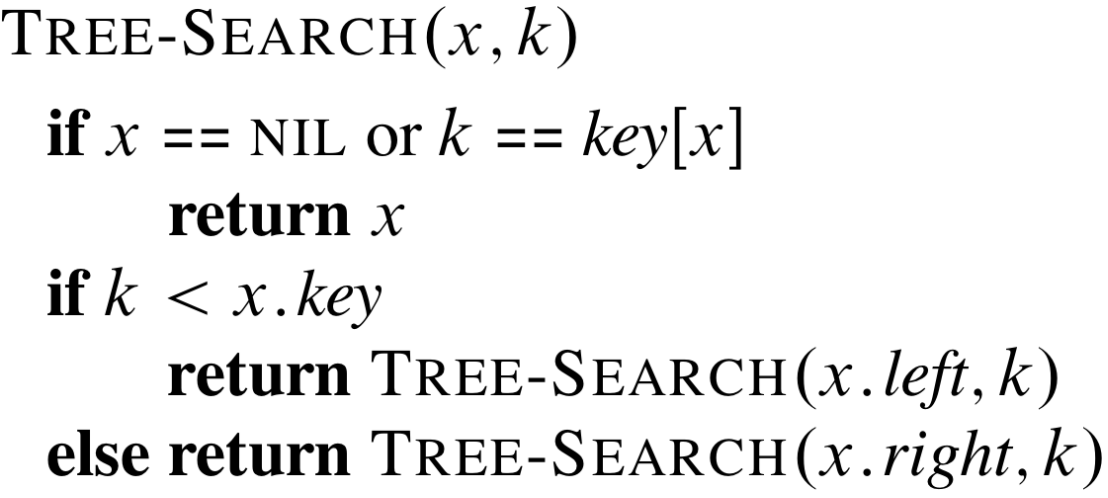
\includegraphics[width=0.85\textwidth]{images/bst-search.png}\\[2pt]
        \textit{Time:} \(O(\log n)\) avg, \(O(h)\) worst\\
        \textit{Space:} \(O(n)\) for tree, \(O(h)\) auxiliary
    \end{minipage}
    \hfill
    \begin{minipage}[t]{0.19\textwidth}
        \centering
        \textbf{\scriptsize BST-Minimum}\\[2pt]
        \scriptsize
        \begin{minipage}[t]{\textwidth}
            \scriptsize
            1. Start at root\\
            2. If NULL, return NULL\\
            3. Follow left pointers until no left child\\
            4. Return leftmost node
        \end{minipage}\\[8pt]
        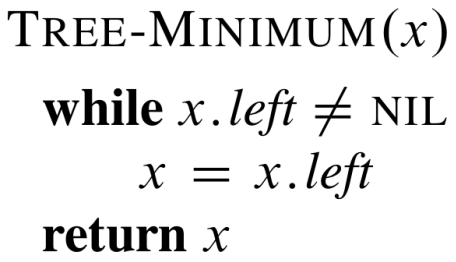
\includegraphics[width=0.5\textwidth]{images/bst-minimum.png}\\[2pt]
        \textit{Time:} \(O(h)\)\\
        \textit{Space:} \(O(n)\) for tree, \(O(1)\) auxiliary
    \end{minipage}
    \hfill
    \begin{minipage}[t]{0.19\textwidth}
        \centering
        \textbf{\scriptsize BST-Maximum}\\[2pt]
        \scriptsize
        \begin{minipage}[t]{\textwidth}
            \scriptsize
            1. Start at root\\
            2. If NULL, return NULL\\
            3. Follow right pointers until no right child\\
            4. Return rightmost node
        \end{minipage}\\[8pt]
        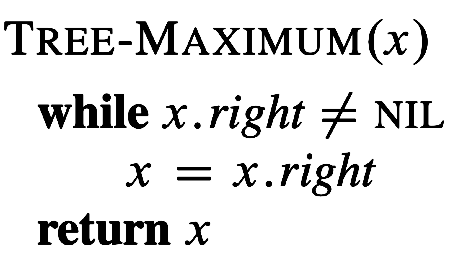
\includegraphics[width=0.5\textwidth]{images/bst-maximum.png}\\[2pt]
        \textit{Time:} \(O(h)\)\\
        \textit{Space:} \(O(n)\) for tree, \(O(1)\) auxiliary
    \end{minipage}
    \hfill
    \begin{minipage}[t]{0.19\textwidth}
        \centering
        \textbf{\scriptsize BST-Successor}\\[2pt]
        \scriptsize
        \begin{minipage}[t]{\textwidth}
            \scriptsize
            1. If right subtree exists:\\
            \quad Return minimum in right subtree\\
            2. Otherwise:\\
            \quad Find first ancestor where\\
            \quad node is in left subtree
        \end{minipage}\\[4pt]
        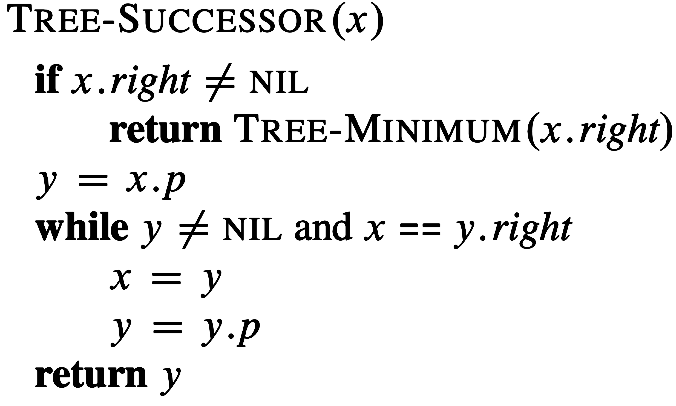
\includegraphics[width=0.8\textwidth]{images/bst-successor.png}\\[2pt]
        \textit{Time:} \(O(h)\)\\
        \textit{Space:} \(O(n)\) for tree, \(O(1)\) auxiliary
    \end{minipage}
    \hfill
    \begin{minipage}[t]{0.19\textwidth}
        \centering
        \textbf{\scriptsize BST-Postorder}\\[2pt]
        \scriptsize
        \begin{minipage}[t]{\textwidth}
            \scriptsize
            1. Recursively traverse left\\
            2. Recursively traverse right\\
            3. Visit current node\\
            \textit{(Children first, then root)}
        \end{minipage}\\[4pt]
        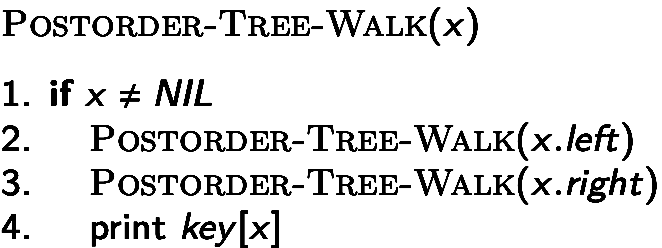
\includegraphics[width=0.8\textwidth]{images/bst-postorder.png}\\[2pt]
        \textit{Time:} \(O(n)\)\\
        \textit{Space:} \(O(n)\) for tree, \(O(h)\) auxiliary
    \end{minipage}
    \hfill
    \begin{minipage}[t]{0.19\textwidth}
        \centering
        \textbf{\scriptsize BST-Inorder}\\[2pt]
        \scriptsize
        \begin{minipage}[t]{\textwidth}
            \scriptsize
            1. Recursively traverse left\\
            2. Visit current node\\
            3. Recursively traverse right\\
            \textit{(Visits nodes in sorted order)}
        \end{minipage}\\[4pt]
        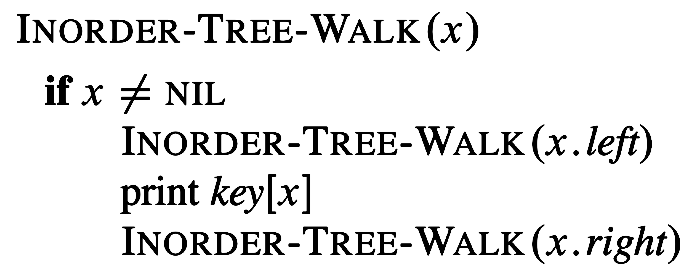
\includegraphics[width=0.8\textwidth]{images/bst-inorder.png}\\[2pt]
        \textit{Time:} \(O(n)\)\\
        \textit{Space:} \(O(n)\) for tree, \(O(h)\) auxiliary
    \end{minipage}
    \hfill
    \begin{minipage}[t]{0.19\textwidth}
        \centering
        \textbf{\scriptsize BST-Preorder}\\[2pt]
        \scriptsize
        \begin{minipage}[t]{\textwidth}
            \scriptsize
            1. Visit current node\\
            2. Recursively traverse left\\
            3. Recursively traverse right\\
            \textit{(Root first, then children)}
        \end{minipage}\\[4pt]
        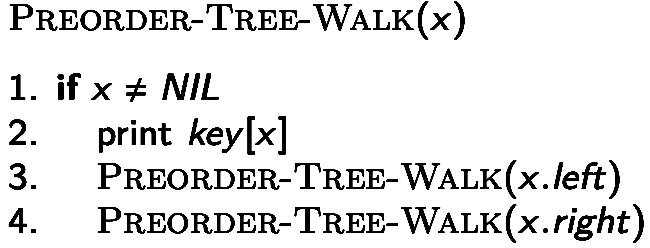
\includegraphics[width=0.8\textwidth]{images/bst-preorder.png}\\
        \textit{Time:} \(O(n)\)\\
        \textit{Space:} \(O(n)\) for tree, \(O(h)\) auxiliary
        \begin{minipage}[t]{1.6\textwidth}
        \hrule
        \end{minipage}
        \vspace{2pt}
        \textbf{Properties:}\\
        \begin{minipage}[t]{1.6\textwidth}
            \begin{itemize}
            \item[-] Left subtree: all keys < node's key
            \item[-] Right subtree: all keys > node's key
            \item[-] Left and right subtrees are also BSTs
            \item[-] A \textbf{Node} has: \textbf{key} (value), \textbf{left} \& \textbf{right} (child pointers), \textbf{parent} (optional)
            \item[-] Tree height \textbf{h}: length of longest path from root to leaf
            \end{itemize}
        \end{minipage}
    \end{minipage}
    \hfill
    \begin{minipage}[t]{0.19\textwidth}
        \centering
        \textbf{\scriptsize BST-Insert}\\[2pt]
        \scriptsize
        \begin{minipage}[t]{\textwidth}
            \scriptsize
            1. Create new node z with key\\
            2. Start at root, track parent y = NIL\\
            3. Move down tree (left if key < node key, right otherwise)\\
            4. Once NULL found, link z as child of y\\
            5. If y is NIL, z becomes root\\
            6. Otherwise, insert z as left or right child based on key comparison
        \end{minipage}\\[4pt]
        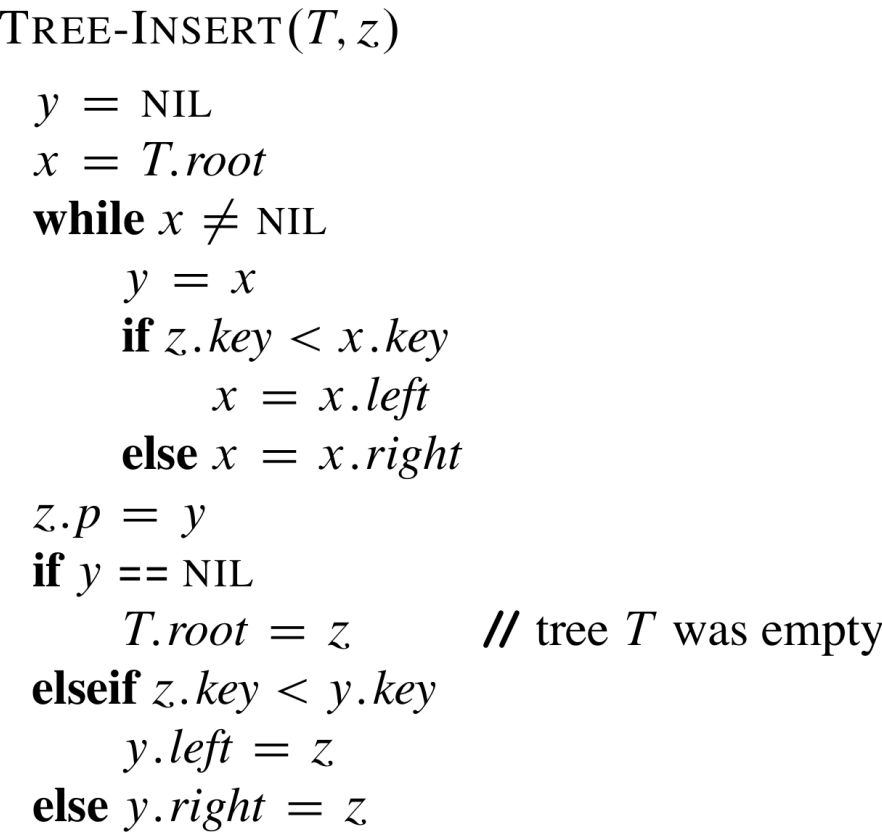
\includegraphics[width=0.8\textwidth]{images/bst-insert.png}\\[2pt]
        \textit{Time:} \(O(h)\)\\
        \textit{Space:} \(O(n)\) for tree, \(O(1)\) auxiliary
    \end{minipage}
    \hfill
    \begin{minipage}[t]{0.19\textwidth}
        \centering
        \textbf{\scriptsize BST-Transplant}\\[2pt]
        \scriptsize
        \begin{minipage}[t]{\textwidth}
            \scriptsize
            Replace subtree at u with v:\\
            1. If u is root, set v as root\\
            2. If u is left child, make v left child of u's parent\\
            3. Else make v right child of u's parent\\
            4. Set v's parent to u's parent
        \end{minipage}\\[4pt]
        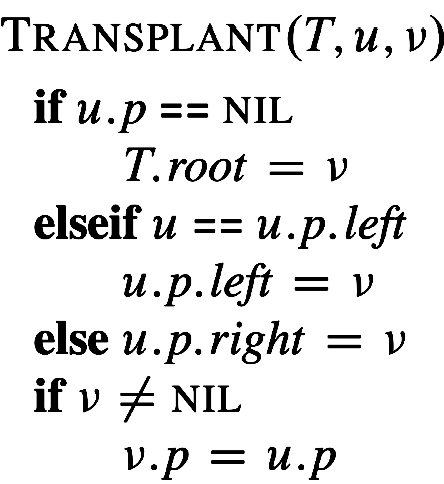
\includegraphics[width=0.4\textwidth]{images/bst-transplant.png}\\[2pt]
        \textit{Time:} \(O(1)\)\\
        \textit{Space:} \(O(n)\) for tree, \(O(1)\) auxiliary
    \end{minipage}
    \hfill
    \begin{minipage}[t]{0.19\textwidth}
        \centering
        \textbf{\scriptsize BST-Delete}\\[2pt]
        \scriptsize
        \begin{minipage}[t]{\textwidth}
            \scriptsize
            1. If z has no left: transplant right\\
            2. If z has no right: transplant left\\
            3. With both children:\\
            \quad a. Find successor y\\
            \quad b. Handle y's children\\
            \quad c. Replace z with y
        \end{minipage}\\[4pt]
        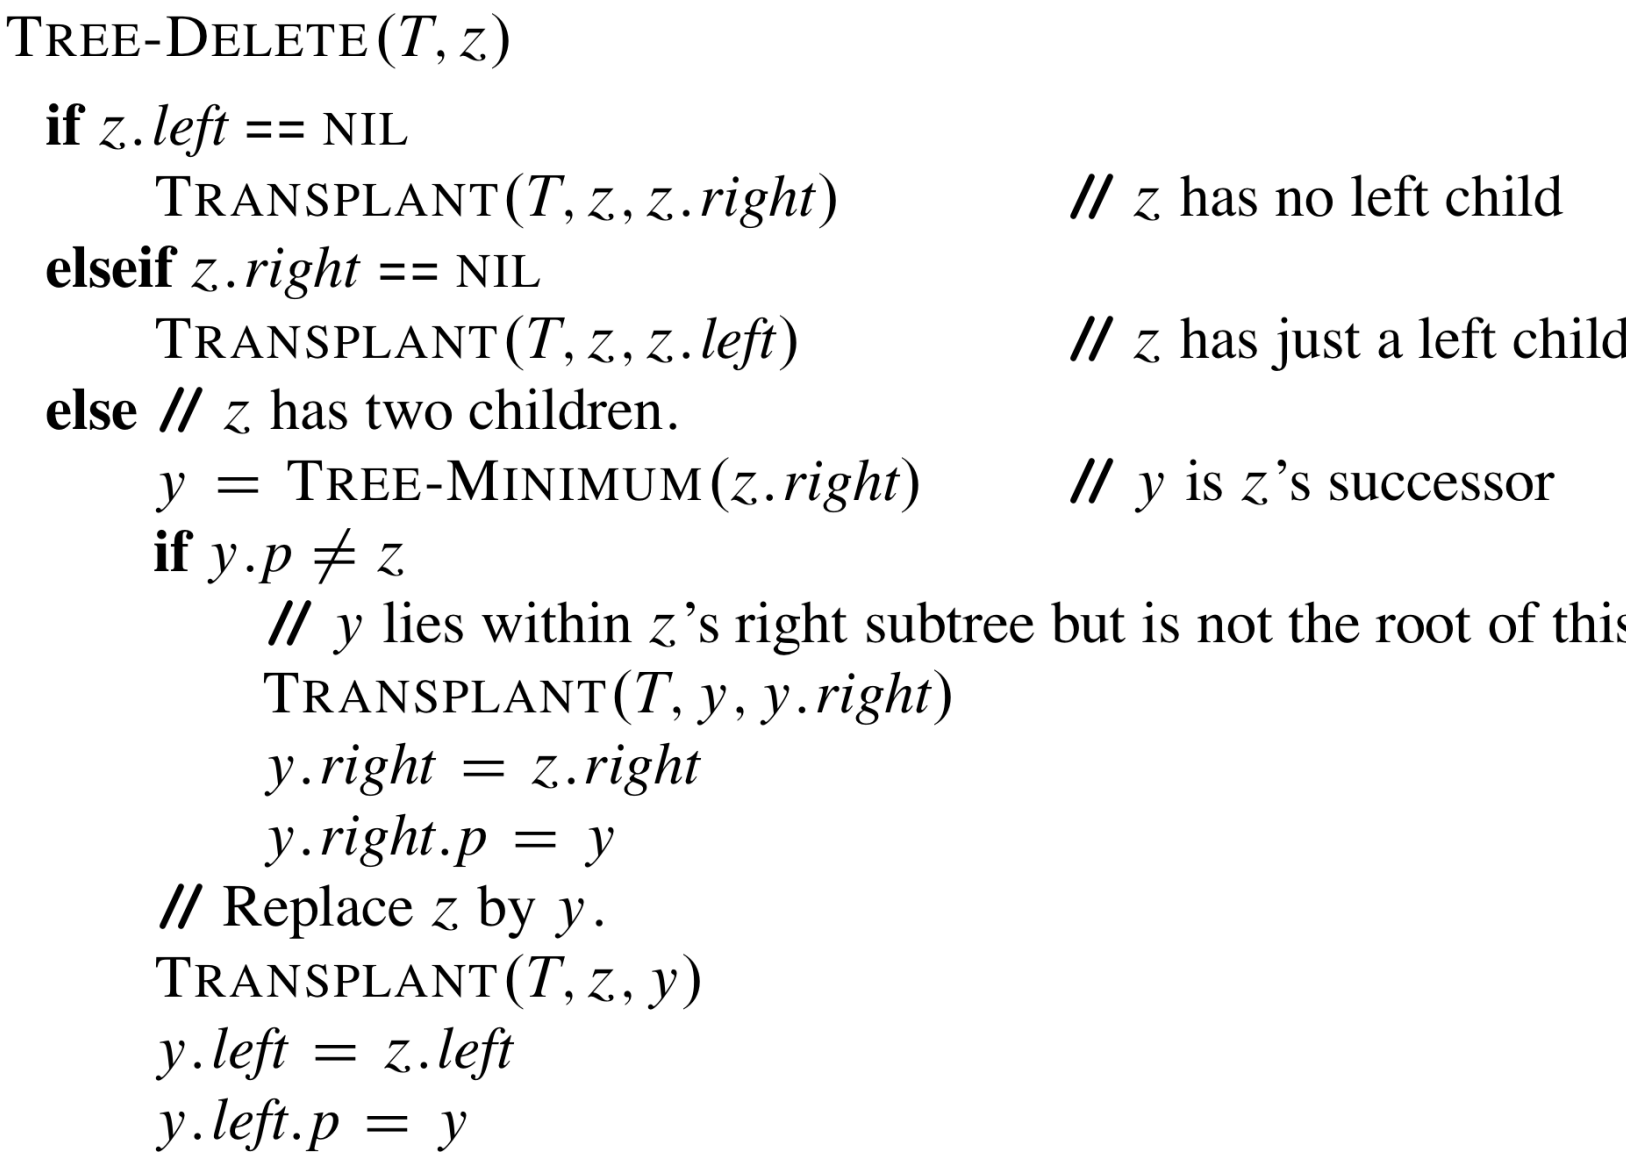
\includegraphics[width=1\textwidth]{images/bst-delete.png}\\[2pt]
        \textit{Time:} \(O(h)\)\\
        \textit{Space:} \(O(n)\) for tree, \(O(1)\) auxiliary
    \end{minipage}
    
    \vspace{2pt}
\end{minipage}} 